
\documentclass[fleqn]{hw}

\usepackage{notes}
\usepackage{url}
\usepackage{graphicx}
\usepackage{amsmath}
\usepackage{float}
\topmargin -1.5cm        % read Lamport p.163
\oddsidemargin -0.04cm   % read Lamport p.163
\evensidemargin -0.04cm  % same as oddsidemargin but for left-hand pages
\textwidth 16.59cm
\textheight 21.94cm
\parskip 7.2pt           % sets spacing between paragraphs

\newcommand{\indep}{\perp}

\title{HW5: Bayesian Networks \& Independence}
\class{CS6300: Artificial Intelligence, Spring 2018}
\institute{University of Utah}
\author{Jake Pitkin}
% IF YOU'RE USING THIS .TEX FILE AS A TEMPLATE, PLEASE REPLACE
% The author WITH YOUR NAME AND UID.
% Replace the due date with anyone you worked with i.e. "Worked with: John McCarthy, Watson, & Hal-9000"
\begin{document}
\maketitle

\section{Independences from Probability Tables}

\begin{table}[H]
\centering	
\begin{tabular}{|ccc|c|}
\hline
{\bf A} & {\bf B} & {\bf C} & $p$ \\
\hline
T & T & T & $1/16$ \\
T & T & F & $1/3$ \\
T & F & T & $1/32$ \\
T & F & F & $1/12$ \\
F & T & T & $3/16$ \\
F & T & F & $1/6$ \\
F & F & T & $3/32$ \\
F & F & F & $1/24$ \\
\hline
\end{tabular}
\caption{$P(A, B, C)$}
\end{table}

I considered a few factorizations and found one that satisfied the above table.

\begin{center}
	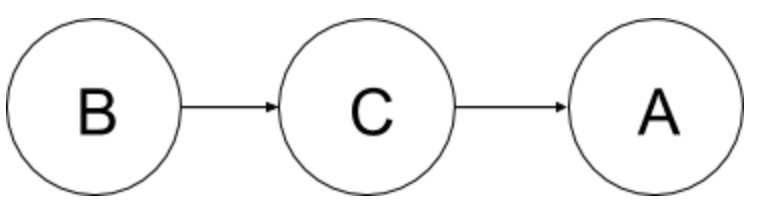
\includegraphics[width=0.25\textwidth]{p1}
\end{center}

This factorizes the joint probability $P(A, B, C)$ as a product of the conditional probabilities $P(B)$, $P(C | B)$, and $P(A | C)$. 

\begin{table}[H]
        \begin{minipage}{0.333\textwidth}
            \centering
            \begin{tabular}{|c|c|}
\hline
{\bf B} & $p$ \\
\hline
T & $3/4$ \\
F & $1/4$ \\
\hline
\end{tabular}
\caption{$P(B)$}
        \end{minipage}
        \hfillx
        \begin{minipage}{0.3333\textwidth}
            \centering
      \begin{tabular}{|cc|c|}
\hline
{\bf C} & {\bf B} & $p$ \\
\hline
T & T & $1/3$ \\
T & F & $1/2$ \\
F & T & $2/3$ \\
F & F & $1/2$ \\
\hline
\end{tabular}
\caption{$P(C | B)$}
        \end{minipage}
        \begin{minipage}{0.333\textwidth}
            \centering
\begin{tabular}{|cc|c|}
\hline
{\bf A} & {\bf C} & $p$ \\
\hline
T & T & $1/4$ \\
T & F & $2/3$ \\
F & T & $3/4$ \\
F & F & $1/3$ \\
\hline
\end{tabular}
\caption{$P(A | C)$}
        \end{minipage}
    \end{table}
    
With 10 total entries, this is the smallest you can get the conditional probability tables (keeping the graph connected). These were derived by marginalizing out variables from $P(A, B, C)$ and using the product rule for dependent variables.

\newpage
\section{Independence in Graphical Models}

Consider the graphical model shown below:

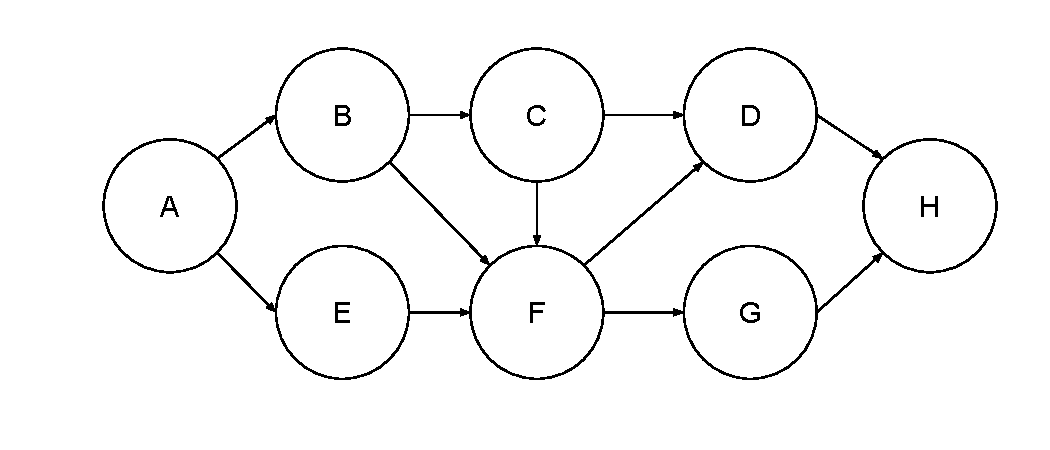
\includegraphics[width=0.5\textwidth]{example-network}

Please answer the following conditional independence questions from
this model:

\begin{enumerate}
\item $A \indep H$
\item $A \indep H | C$
\item $A \indep H | C,F$
\item $E \indep B | A$
\item $E \indep B | C,F$
\item $E \indep B | A,C,F$
\end{enumerate}

\newpage
\section{Inference by Enumeration and Variable Elimination}

Consider the graphical model for the alarm network.  Using inference by enumeration, compute the
following probabilities (show your work!!!):

\begin{enumerate}
\item $p(b, \lnot e | a, j, m)$
\item $p(b | a)$
\item $p(b | e,a)$  (how does this compare to the previous one?)
\item $p(a | j,\lnot m)$
\end{enumerate}

Now, repeat items (2) and (4) using variable elimination.  When you
have to choose a variable to eliminate, choose alphabetically.


\end{document}
